\chapter{The Standard Model, the Higgs Boson and New Scalar Particles}

\section{Phenomenology of the Standard Model}


The Standard Model (SM) of particle physics~\cite{Halzen:1984mc} is a description of nature which best explain  our understanding of the fundamental structure of matter and the fundamental forces which govern all known phenomena. The SM gives a quantitative description of three of the four interactions in nature: electromagnetism, weak interactions and the strong nuclear force.
Developed in the early 1970s by Glashow~\cite{GLASHOW1961579}, Weinberg~\cite{PhysRevLett.19.1264} and Salam~\cite{Salam:1968rm}, it has successfully explained almost
all experimental results and precisely predicted a wide variety of phenomena.
It is a renormalizable quantum field theory, compatible with special relativity.

\subsection*{General Picture}
The main constituents of the SM and  are shown in Fig.~\ref{SM}. These  are the particles that composed the ordinary matter.
\begin{figure}
\centering
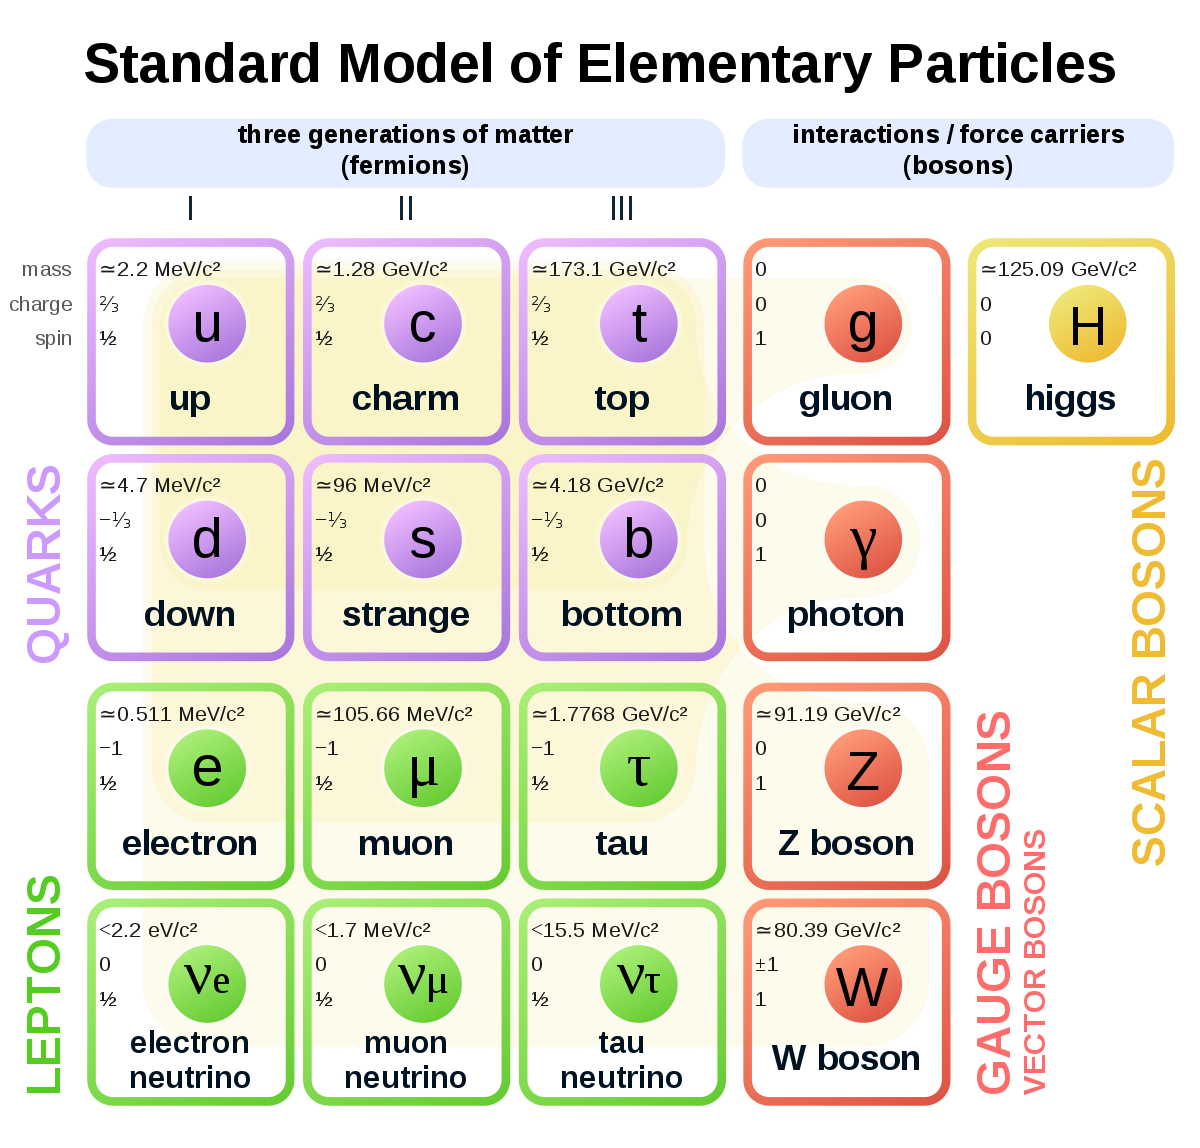
\includegraphics[scale= 0.2]{../Cap1/SM}
\caption{Main constituents of the Standard Model.}
\label{SM}
\end{figure}
The particles involved are characterized by the spin, the mass, and the quantum numbers determining their interactions.
The quarks are subject to all the three forces and, in particular, are the only fermions to
possess a ``colour'' charge to which QCD. Because of the QCD colour confinement properties, quarks do not exist as free states
but can be experimentally observed only as bound states. All system composed by quark haven't a color charge. The proton and neutron, that constituent the ordinary matter, are composed by three quarks (called baryons). The particle composed by a quark-antiquark are called ``meson''. Quark flavour is conserved in electromagnetic and strong interactions but not in weak ones, as quark mass eigenstates do not correspond to the weak interaction eigenstates.
Their mixing is described by the Cabibbo–Kobayashi–Maskawa (CKM) matrix.
The leptons have no colour charge and are subject only to the electromagnetic and weak
forces. The charged leptons of the three families are respectively denoted as the electron
(e), muon ($\mu$) and tau lepton ($\tau$). The only stable lepton is the electron. To each lepton corresponds a neutrino. The mass of neutrino is unknown and their flavour oscillations prove a non-zero mass~\cite{Balantekin:2013tqa}. 
The gluons, the W$^{\pm}$ bosons, the Z boson and the photon $\gamma$ are boson that compose the SM gauge sector.
The gluons are the mediators of the strong interactions. They are massless, electrically neutral and carry color quantum number and they can interact with themselves.
The  W$^{\pm}$ and Z bosons are the mediate the weak interactions. Their mass is $\sim$81 GeV and $\sim$90 GeV respectively. These particles are unstable and after their production decay in other particles. Finally the photon is massless, chargeless and non self-interacting and mediates the electromagnetic
interactions.
The SM Lagrangian may be written as the sum of three parts:
\begin{equation}
 \mathcal{L}_{SM} = \mathcal{L}_{QCD}+\mathcal{L}_{EWK}+\mathcal{L}_{H}    \end{equation}
where $\mathcal{L}_{QCD}$ is the quantum chromodynamics Lagrangian that describes the interactions of quarks and gluons, the $\mathcal{L}_{EWK}$ is the the electroweak Lagrangian that describes the interactions from the fermions with the $Z$ and  W$^{\pm}$ bosons. The $\mathcal{L}_{H}$ is the Higgs part of the Lagrangian: the Lagrangian symmetries, seem to forbid the introduction of mass terms without spoiling its gauge invariance. Higgs’ proposal solves this problem by spontaneously breaking the Lagrangian symmetry (Sec.~\ref{H}).


\subsection*{Experimental evidence}
The experimental study  of the Standard Model  has made a quantum leap in the last 30 years. First of all the theory was predicted the existence of W$^{\pm}$ and Z bosons in the mass range from 60 to 93 GeV~\cite{doi:10.1142/9789814644150_0006}. 
In 1976 Rubbia, Cline and McIntyre proposed the transformation of an existing high-energy proton accelerator at  into a proton–antiproton collider as a quick and relatively cheap way to achieve collisions above threshold for W and Z production.  It was adopted at CERN (SPS) and the first  proton–antiproton
 collisions was collected in 1981. In the following years the W and Z bosons have been observed by UA1 and UA2 experiments with a mass of 80 GeV and 91 GeV respectively, Fig.~\ref{rubbia_f}. 
\begin{figure}
\centering%
\subfigure[]%
{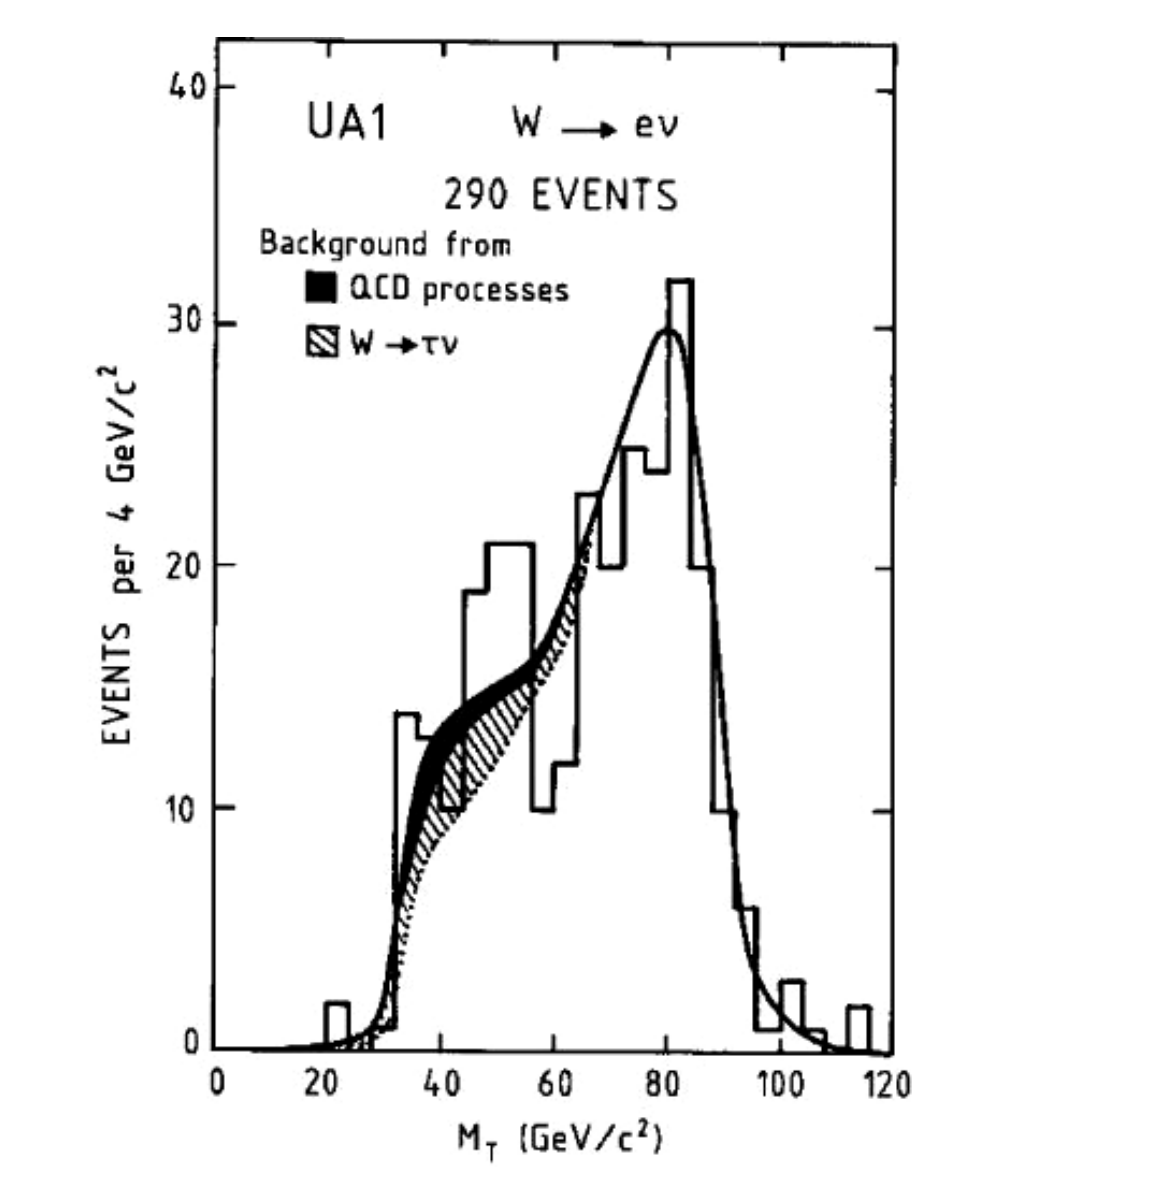
\includegraphics[scale= 0.66]{../Cap1/rubbia_W}}
\subfigure[]%
{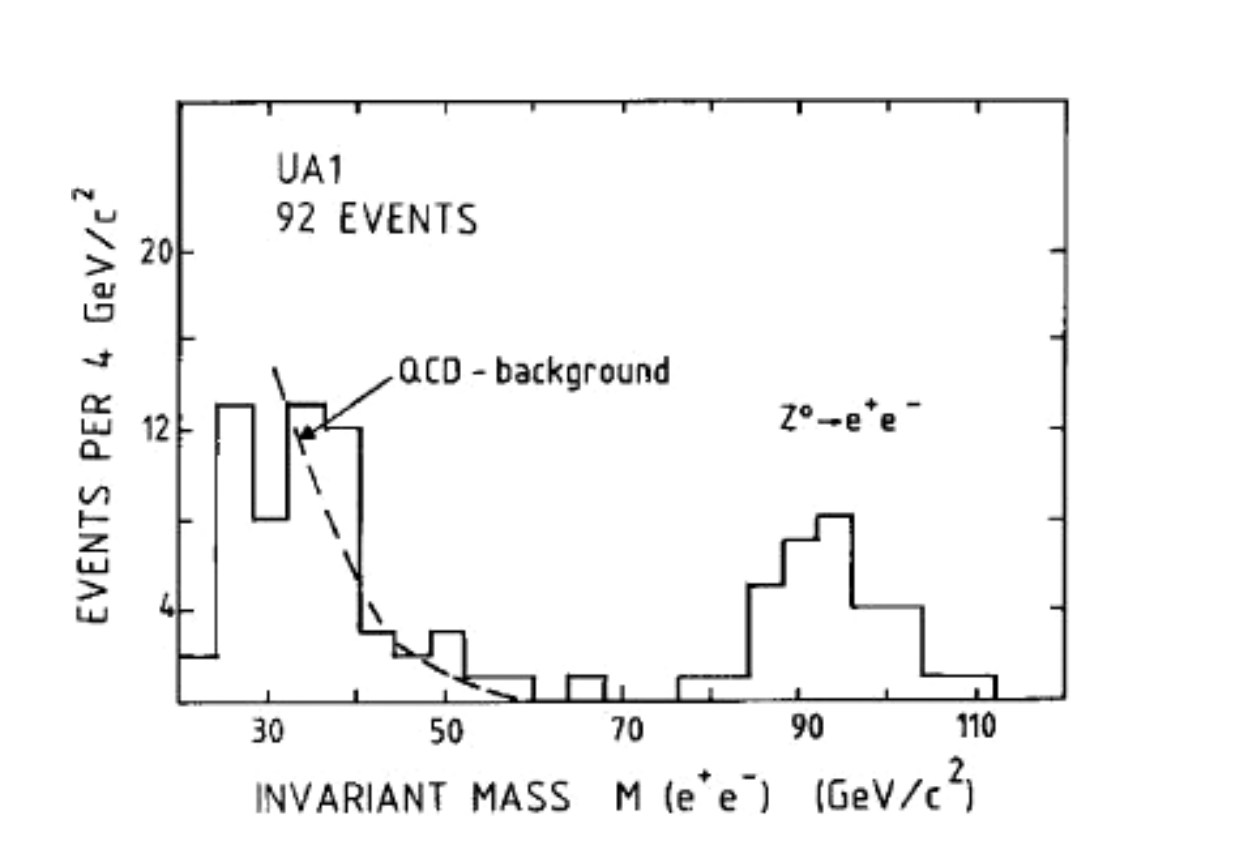
\includegraphics[scale= 0.66]{../Cap1/rubbia_Z}}
\caption{(a) Transverse mass distribution for all W$\to e \nu$ events recorded by UA1 between 1982 and 1985. (b) Invariant mass distribution of all $e^+e^-$
pairs recorded by UA1 between 1982 and 1985}
\label{rubbia_f}
\end{figure}
With the advent of electron-positron colliders, for the first time, precise measurements of the fundamental parameters of electroweak theory could be made. 
In 1989, two $e^+e^-$ colliders commenced operations on far away sides of the world:
the Stanford Linear Collider (SLC) at SLAC,  and the circular Large Electron
Positron collider (LEP) at CERN. Precision electroweak tests covering the measurements at the Z pole and W boson properties, i.e. cross section for W-pair production is shown, have been conducted by SLD and LEP experiments, Fig.~\ref{alt}. The results of measurements confirmed the SM prediction. 
\begin{figure}
\centering%
\subfigure[]%
{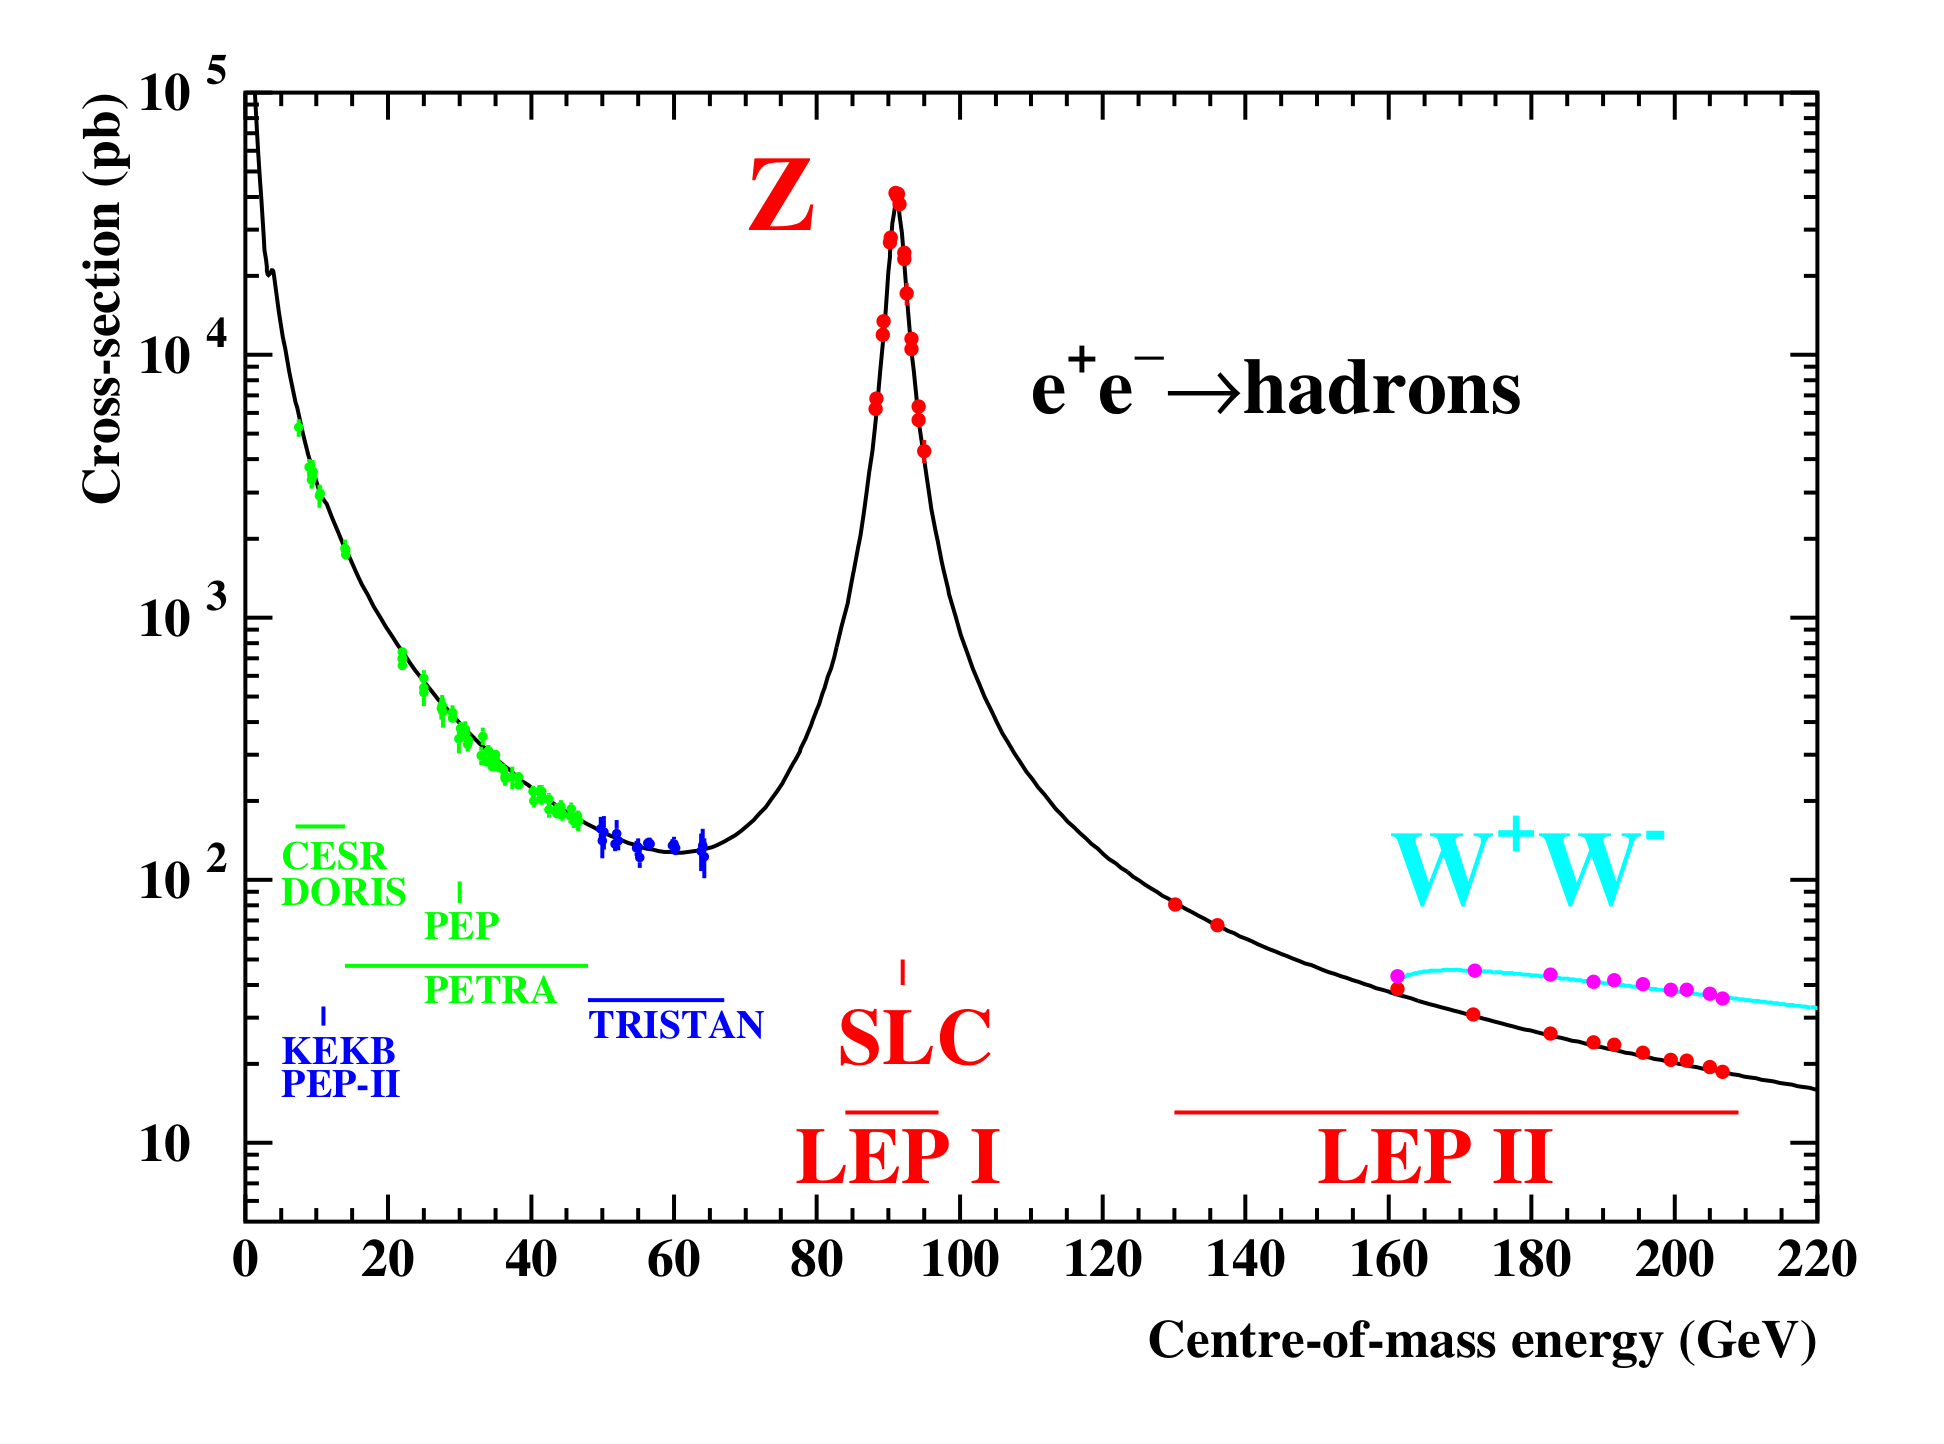
\includegraphics[scale= 0.4]{../Cap1/alt_Z}}
\subfigure[]%
{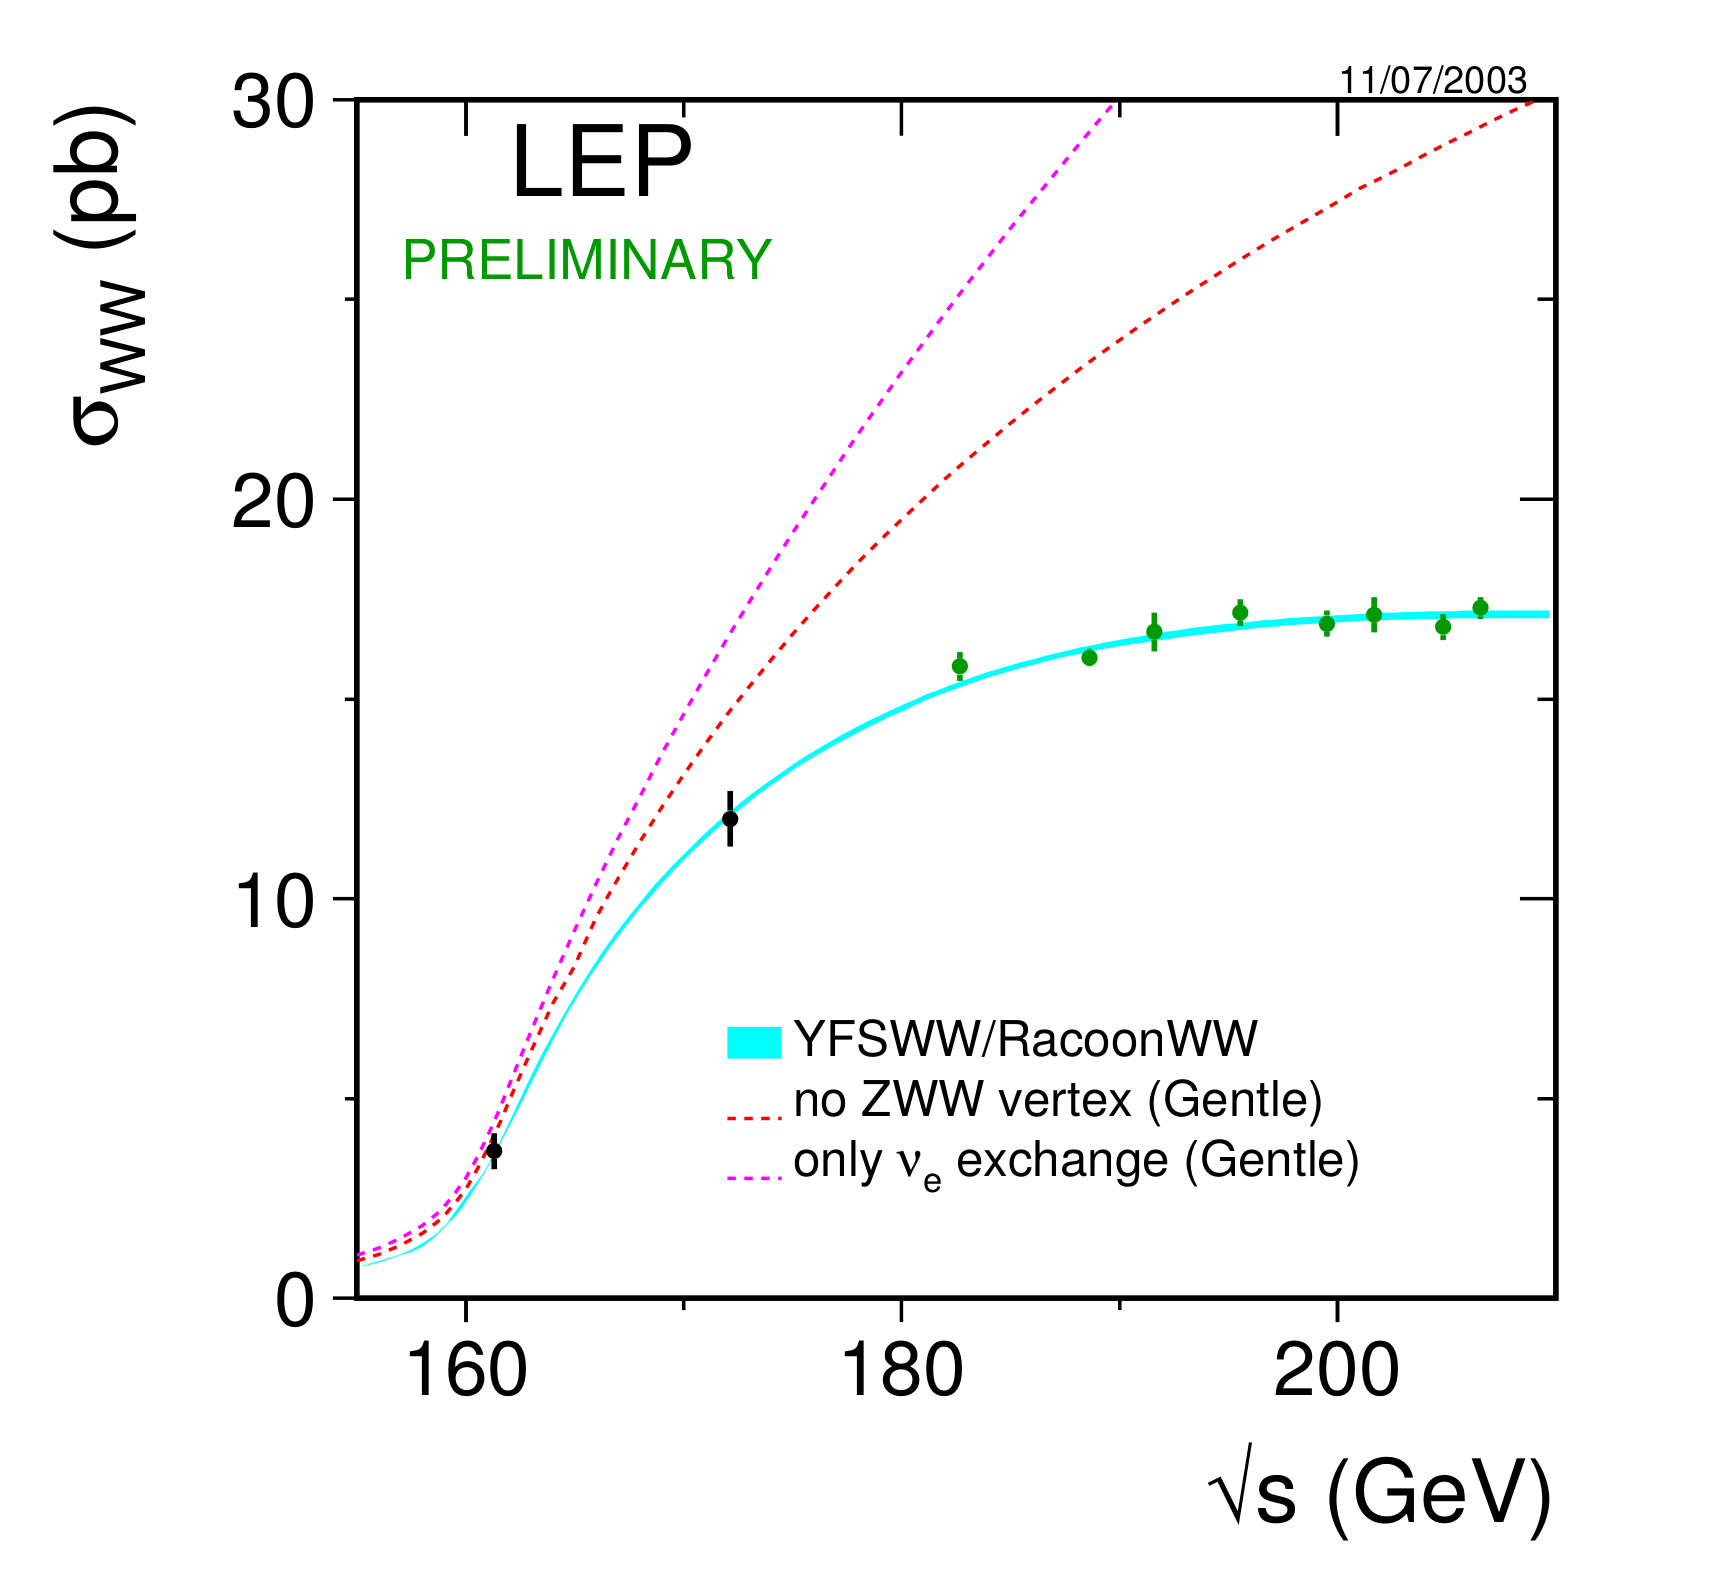
\includegraphics[scale= 0.4]{../Cap1/alt_W}}
\caption{(a) The cross-section for the production of hadrons in $e^+e^-$ annihilations. The measurements are shown as dots with error bars. The solid line shows the prediction of the SM. (b) The measured W-pair production cross section compared to the SM and alternative
theories not including trilinear gauge couplings.}
\label{alt}
\end{figure}
The next missing SM piece was top quark evidence. It was a necessary component of the SM of electroweak interactions, but there was no consistent theoretical guidance as to what its mass should be. The only way to observe a top quark with such a high mass was at the collider with the highest-energy, the Tevatron antiproton-proton collider at Fermilab. The existence of the top quark was firmly established in 1995 with simultaneous announcements by both the CDF~\cite{PhysRevLett.73.225} and the DO~\cite{D0:1995jca} experiments of results that demonstrated a mass of around 174 GeV, Fig.\ref{Wells2004_Article_ExperimentalTestsOfTheStandard}.
After the top quark discovery, the only missing part to the SM is the Higgs boson particle  that has been observed at ATLAS and CMS experiment at LHC proton-proton collider at CERN in 2012 (see Sec.\ref{H}).  
\begin{figure}
\centering
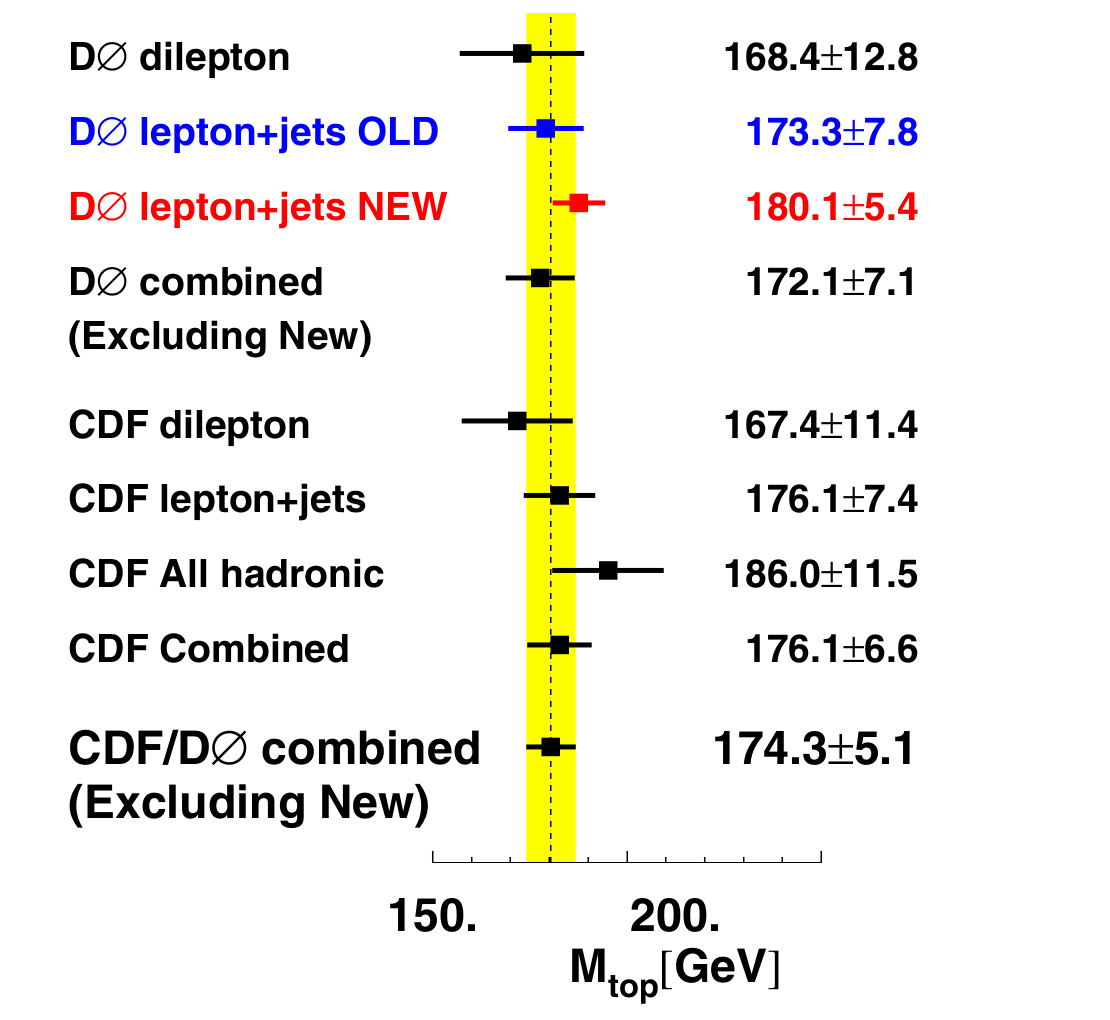
\includegraphics[scale= 0.66]{../Cap1/Wells2004_Article_ExperimentalTestsOfTheStandard}
\caption{Top quark mass measurements.}
\label{Wells2004_Article_ExperimentalTestsOfTheStandard}
\end{figure}


\subsection*{Open Questions} The Standard Model is now the best description of the subatomic nature, but this theory does not explain the complete picture of the world. Sure enough there are more open questions: the gravity is not described in the model, the explanation of the dark matter is not clear and the knowledge of neutrino mixing and mass are not very understood.
The gravity is one of the four fundamental interaction but it is not described in the  SM. It is so different from the three other
forces and the purpose to establish a common theory that describe all forces is so difficult. The gravity is described in the  Einstein’s General Relativity (GR) theory. To combine the  SM with the GR it is necessary a quantum theory with a new field associated to gravity that has as mediator a spin 2 particle called graviton. Right now there are no experimental evidence of the existence of this kind of particle. The other deficit of the SM regarding the dark matter, in fact, from astronomical observations, only the 5\% of the  matter and energy content of our universe is formed by the ordinary matter (hadrons and leptons), the other 95\% is composed by dark matter and dark energy. The SM does not offer good candidates or explainations for the dark matter and dark energy problems although some research at colliders have been done.
Regarding the neutrino, in the SM they were assumed massless. However the fact that
neutrinos have a  flavour oscillation implies that they must have non zero mass differences.
It is not clear that the small neutrino masses  can arise from the same electroweak symmetry breaking mechanism that
is in act for the other SM particles.



\section{The Higgs Boson}
\label{H}
A symmetrical Lagrangian is invariant under a group of transformations. However the fact that the weak gauge bosons have a mass different from zero indicates that
the electroweak Lagrangian, $\mathcal{L}_{EWK}$, is not a symmetry of the vacuum. Also the fermion masses can
not be included without violating gauge symmetry in the $\mathcal{L}_{QCD}$.
The mass terms can be introduced with the Spontaneous Symmetry Breaking Mechanism, adding  $\mathcal{L}_{H}$, that gives mass to the weak bosons and fermions and leaves the photon massless. 

\subsection*{The Brout–Englert–Higgs mechanism}
The symmetry of SM Lagrangian, $\mathcal{L}_{SM}$, is $SU(2) \otimes U(1)$. To broken symmetry group,  a  scalar field $\Phi$ (Higgs field) is introduced. The field is a doublet isospin ($SU(2)_L$) as,
\newline
$$
\Phi=
\left(
\begin{array}{c}
\Phi^+   \\
\Phi^0 \\
\end{array}
\right)
=\frac{1}{\sqrt{2}}
\left(
\begin{array}{c}
\Phi_1 + i\Phi_2   \\
\Phi_3 + i\Phi_4  \\
\end{array}
\right)
$$
where $\Phi_j$ with $j=1,2,3,4$ are real fields used to manifest the complexity of $\Phi^+$ and  $\Phi^0$. The simplest Lagrangian of a self-interacting scalar field is in the form of,
\begin{equation}
 \mathcal{L}_{H}= (D^{\mu} \Phi^{\dag})(D_{\mu} \Phi) -\mu^2 \Phi^{\dag}\Phi - \lambda(\Phi^{\dag}\Phi)^2 \end{equation}
where $\lambda$ needs to be positive for the potential to be bounded from below and $\mu^2$
 is a mass term for the $\Phi$ field.
The ground state (vacuum) of the theory is defined as the state where the energy density is at a minimum.
If the $\mu$ parameter is chosen so that $\mu^2<0$, the symmetry of the potential may be broken,
as it has a minimal value of,
\newline
$$
v\equiv
\sqrt{\frac{-\mu^2}{\lambda}}
$$
This is illustrated in Fig.~\ref{higgspotential}.

\begin{figure}
\centering
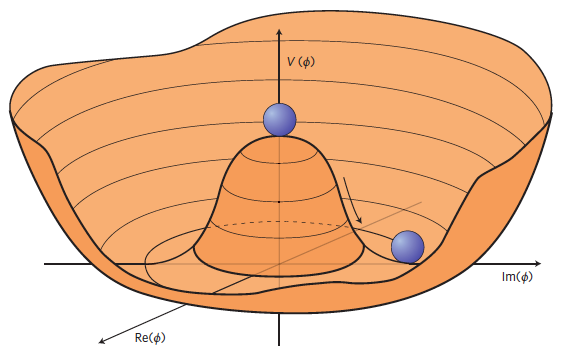
\includegraphics[scale= 0.4]{../Cap1/higgspotential}
\caption{Higgs fields potential.}
\label{higgspotential}
\end{figure}


\subsection*{The Higgs boson at colliders}

\subsection*{Experimental Results}

\subsection*{Higgs boson to WW channel}

\section{New Scalar Particles}
There are many deficiencies of the Standard Model (SM), such as the hierarchy problem,
flavor problem, dark matter problem, cosmological constant problem, electroweak symmetry breaking problem, CP violation problem, baryogenesis problem, etc.
The presence of a hidden sector, defined here to mean extra states that
have no SM gauge charge but are charged under some other exotic gauge symmetry, does not necessarily solve any of the problems above. However, in order to identify whether the SM Higgs sector is complete,  the searches of additional heavy scalars are performed.  They would prove the presence of beyond-the-SM (BSM) physics in the form of a non-minimal Higgs sector~\cite{Robens:2015gla}. The existence of sibling Higgs boson, denoted X, is motivated in many BSM scenarios, so the research in the full mass range accessible at colliders  remains one of the main objectives of the experimental community. This  road  needs  to  be continued within the full mass range that is accessible to current and future experiments.
\newline
\subsection*{Higgs Singlet Extension}
The simplest extension of the SM Higgs sector consist in an additional singlet which is neutral under all quantum number of the SM gauge groups.
A complex $SU(2)_L$ doublet,  denoted $\Phi$, is added by an additional real scalar $S$ which is a singlet under all SM gauge groups. 
The most general gauge-invariant and renormalisable scalar Lagrangian is,


\begin{equation}
 \mathcal{L}_s = (D_{\mu} \Phi )^{\dagger}  \: D_{\mu} \Phi  +  \partial^{\mu}S   \partial_{\mu}S -V(\Phi, S)     \end{equation}
where $V(\Phi, S) $ is the scalar potential,  

\begin{equation}
 V(\Phi, S)= -m^2   \Phi ^{\dagger}\Phi -\mu^2 S^2 +\lambda_1 (\Phi ^{\dagger}\Phi)^2 +\lambda_2 S^4 + \lambda_3 \Phi ^{\dagger}\Phi^2 S^2  \end{equation}
Here, $Z_2$ ($S \rightarrow -S$) symmetry is imposed which forbids additional terms in the potential.
The scalar potential $V(\Phi, S)$ is bounded from below if the following conditions are fulfilled,

\begin{equation}
 4 \lambda_1  \lambda_2 - \lambda_3^2 >0    \end{equation}

\begin{equation}
 \lambda_1 , \lambda_2  >0    \end{equation}

where if the first condition is fulfilled, the extremum is a local minimum. The
second condition (5), guarantees that the potential is bounded from below for large field values.
The Higgs fields, $\Phi$ and $S$, have non-zero vacuum expectation, denoted by $v$ and $x$, respectively.
Following the unitary-gauge prescription, the the Higgs fields is given by,
\newline
$$
{\mathcal H} \equiv \left(
\begin{array}{c}
0  \\
\frac{\tilde{h}+v }{\sqrt{2}}  \\
\end{array}
\right)
, \qquad 
S \equiv \frac{h'+x }{\sqrt{2}}
.
$$
Expansion around the minimum leads to the squared mass matrix
\newline
$$
{\mathcal M}^2 = \left(
\begin{array}{cc}
2 \lambda_1^2 v^2 & \lambda_3 vx  \\
\lambda_3 vx & 2 \lambda_1^2 x^2 \\

\end{array}
\right)
$$
\newline
with the mass eigenvalues

\begin{equation}
 m_h^2=  \lambda_1 v^2 + \lambda_2 x^2 -\sqrt{(\lambda_1 v^2 - \lambda_2 x^2)^2 +\lambda_3 (xv)^2 } \qquad,  \end{equation}

\begin{equation}
 m_H^2=  \lambda_1 v^2 + \lambda_2 x^2 +\sqrt{(\lambda_1 v^2 - \lambda_2 x^2)^2 +\lambda_3 (xv)^2 } \qquad,  \end{equation}
\newline
where $h$ and $H$ are the scalar fields of definite masses $m_h$ and $m_H$ respectively, with $m_h^2 < m_H^2$ .
The gauge and mass eigenstates are related via the mixing matrix
\newline
$$
\left(
\begin{array}{c}
h   \\
H \\
\end{array}
\right)
=
\left(
\begin{array}{cc}
\cos \alpha & -\sin \alpha   \\
\sin \alpha & \cos \alpha \\
\end{array}
\right)
\;
\left(
\begin{array}{c}
\tilde{h}   \\
h' \\
\end{array}
\right)
$$
\newline
where the mixing angle $ - \frac{\pi}{2} \leq \alpha \leq  \frac{\pi}{2} $ is given by,
\newline
\begin{equation}
\sin 2 \alpha= \frac{\lambda_3 xv}{\sqrt{(\lambda_1 v^2 - \lambda_2 x^2)^2 +\lambda_3 (xv)^2 } } \; , \end{equation}


\begin{equation}
\cos 2 \alpha= \frac{\lambda_2 x^2 - \lambda_1 v^2}{\sqrt{(\lambda_1 v^2 - \lambda_2 x^2)^2 +\lambda_3 (xv)^2 } } \; .  \end{equation}
\newline
By the  mixing matrix it is clear that the light (heavy) Higgs couplings to SM particles are now
suppressed by $\cos \alpha $ ( $\sin \alpha $).
The heavy Higgs is a new version of the SM Higgs with rescaled couplings
to the matter contents and to the gauge fields of the SM. In fact, the only novel channel
with respect to the light Higgs case is $H \rightarrow hh$. The partial decay width $\Gamma$ is given by \cite{Schabinger:2005ei},
\newline
\newline
 \begin{equation}
\Gamma_{ H \rightarrow hh} =  \frac{|\mu'|^2}{8 \pi m_H } \, \sqrt{1- \frac{4m_h^2}{m_H^2}}  \; , \end{equation}
\newline
where the coupling strength $\mu'$ is,
\newline
\begin{equation}
 \mu' =  - \frac{\sin 2 \alpha}{2vx} \, (\sin \alpha v + \cos \alpha x) \, (m_h^2 + \frac{m_H^2}{2})  \; . \end{equation}
\newline
In collider phenomenology, is important:
\begin{itemize}
\item the suppression of the production cross section of the two Higgs states induced by the mixing
\item the suppression of the Higgs decay modes to SM particles,
\end{itemize}
For the high mass  scenario, i.e. the case where the heavy Higgs boson is identified with the discovered Higgs state at $\sim$125 GeV, $|\sin \alpha| $= 1 corresponds to the complete decoupling of the second Higgs boson and therefore the SM-like scenario.


\subsection*{Minimal Supersymmetric Standard Model} The simplest extension to the SM, which provides a
framework addressing naturalness, gauge coupling unification, and the existence of
dark matter, is the Minimal Supersymmetric Standard Model (MSSM)~\cite{FAYET1976159}.
Theories where two Higgs fields transform as doublets under $SU(2)_L$ with unit charge $U(1)_Y$, are very interesting. 
The Two Higgs Double Models (2HDMs)~\cite{Barroso:2013zxa} are models that provide
a general effective theory framework for extensions of the electroweak symmetry
breaking sector. In the 2HDMs models, after the EW  symmetry breaking five physical Higgs  particles emerging: 
two neutral CP-even scalars, h, H; one neutral, CP-odd pseudoscalar, A; and two charged scalars, H$^{+}$ and H$^{-}$. All these particles are expected to have a mass at the TeV scale, so in a regime accessible to the particle colliders, as LHC.
The mass spectrum could be divided  in two regions scale: a light Higgs-like particle (h) with mass $m_h= 125$ GeV, and four remaining scalar particle $H$, $A$, $H*{\pm}$, with higher mass and with $m_H \sim m_A \sim m_{H^{\pm}}$.
The Yukawa coupling, in the model with only two Higgs doublets $\Phi_{1,2}$ are~cite{Craig:2012pu},
 \begin{equation}
V_{Yukawa}= - \sum_{i=1,2} (Q \tilde{\Phi_i} \, y_i^{u^{-}}  \bar{u} \, + Q \Phi_i \, y_i^{d} \, \bar{d} + L \Phi_i \, y_i^{e^{-}} e \, + h.c.  )   \; , \end{equation}
where
by convention up-type quarks are always taken to couple to $\Phi_2^0$.
The Glashow-Weinberg condition, that all fermions of a given representation receive their masses through renormalizable
Yukawa couplings, is satisfied by:
\begin{itemize}
\item Type 1, where $y_1^{u,d,e}=0$  (all fermions couple to one doublet).
\item Type 2, where $y_1^u=y_2^d= y_2^e$=0 (the up quark couple to one doublet and the down quarks and leptons couple to the other).
\item Type 3, where $y_1^u=y_1^d= y_2^e$=0 (quarks couple to one doublet and leptons to the other).
\item Type 4, where $y_1^u=y_1^d= y_1^e$=0 (up quark and leptons couple to one doublet and down quarks couple to the other.)
\end{itemize}
Free parameters of the theory are the masses of the  $H$, $A$, $H*{\pm}$ scalars and the angles $\alpha$, $\beta$ that  ully determine the couplings between a single physical Higgs boson and two gauge bosons or two fermions, as well as the coupling between two Higg and a single gauge boson:
\begin{itemize}
\item $\tan \beta =| \Phi_2^0 / \Phi_1^0|$, (expectation value of the ratio among $\Phi_{1,2}^0$).
\item $\alpha$ that is the mixing angle that diagonalizes the $h-H$ mass squared matrix.
\item The four $m_{h,H,A,H^{\pm}}$ masses. 
\end{itemize}
The  wide  range  of  possibilities  for  Higgs  boson  mass  spectrum  hierarchies  and  branching
ratios  in  2HDMs  yields  a  diversity  of  production  and  decay  channels  that  are  relevant  for
multi-lepton  signatures  at  the  LHC.  Multi-lepton  final  states  become  especially  important
when the decay of one Higgs scalar to a pair of Higgs scalars or a Higgs scalar and a vector
boson is possible.  


\subsection*{The $WW$ channel for high mass particle}
Let’s now concentrate on the $X \to WW$ channel, that is the main final state described in the following in the high mass searches.
The two dominant production mechanisms of high mass SM-like Higgs boson are the
gluon gluon fusion and vector boson fusion (VBF) Fig. \ref{prod}. 
The first one is the main mechanism for mass values below 1 TeV, above the VBF production mechanism become more and more important as $m_X$ approaches to high values.
\begin{figure}
\centering
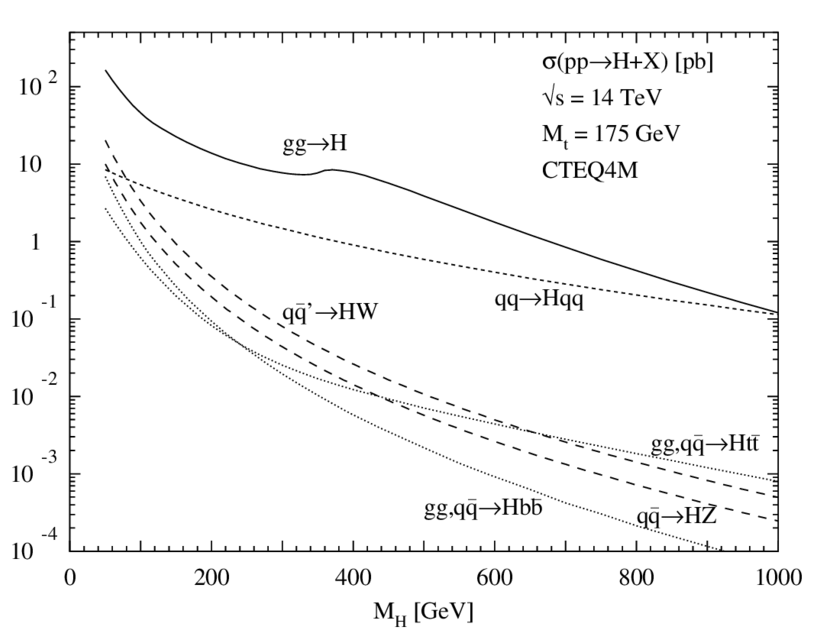
\includegraphics[scale= 0.3]{../Cap1/Higgs-production-cross-sections-at-the-LHC-for-various-production-mechanisms-as-a}
\caption{Higgs-production cross sections at the LHC for various production mechanisms as a function of the Higgs mass. QCD corrections are included except for Higgs bremsstrahlung~\cite{Djouadi2004}.}
\label{prod}
\end{figure}
In the search of high mass Higgs boson for different models scenario, the WW final state, along with ZZ, is the dominant decay channel of $X$ for masses above $2m_Z$ threshold. This fact is evident in Fig. \ref{br} (a), where the $WW$ branching (in green) ratio is dominated in the high mass spectrum. More detailed results on the decays $H \to WW$ and $H \to ZZ $ with the subsequent decay are presented in Fig. \ref{br} (b).
However the yield for the decay channels started by the $X \to WW$ decay is even higher, but the
presence of neutrinos in the final state does not allow to have a completely reconstructed
final state. This fact makes the channel hard to study. 
The gluon gluon fusion production mechanism is characterised by two lepton and two neutrinos in addition to zero or more jets coming from initial state radiation or final state radiation, Sec.~\ref{ps}. The gluon gluon fusion  cross section is between one
and two orders of magnitude larger than that of VBF for a wide range of Higgs masses. Nevertheless, the VBF becomes competitive when the mass approaches to 1 TeV. 
The VBF production, providing two more jets (the VBF jets coming from the hadronization quarks from production) to the final
state, benefits from a highly reduced background with respect to the gluon gluon production mode,
such that even if the VBF production mechanism has a branching ratio smaller than the
gluon-gluon fusion, a higher signal-to-noise ratio is expected.
\begin{figure}
\centering%
\subfigure[]%
{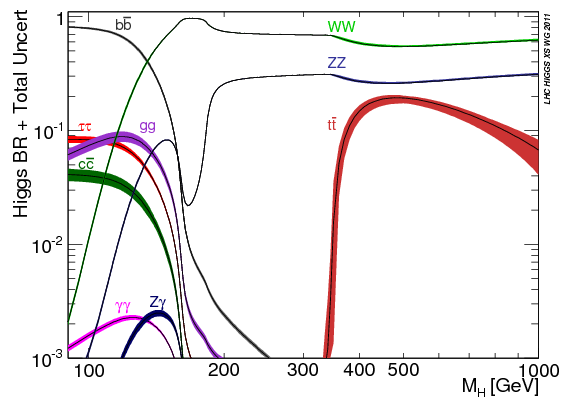
\includegraphics[scale= 0.35]{../Cap1/plots_decay}}
\subfigure[]%
{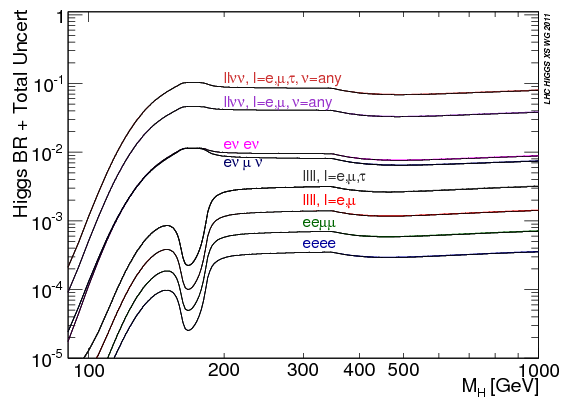
\includegraphics[scale= 0.35]{../Cap1/BRTotalUncertBands4f}}
\caption{(a) Higgs branching ratios and their uncertainties for the full mass range~\cite{Denner:2011mq}. (b) Higgs branching ratios for the different $H \to 4 \ell$ and $H \to 2\ell 2\nu $ final states and their uncertainties for the full mass range~\cite{Denner:2011mq}.}
\label{br}
\end{figure}



\subsection*{$X \to WW$ searches at colliders}
The search of high mass particle with  $WW$ final state  has been widely performed at experiments at hadron
colliders to search for new particles beyond the SM. 
The resonant $WW$ production has been studied at both the Fermilab Tevatron Collider, and the CERN Large
Hadron Collider, with the progressively increasing energy collision and integrated
luminosity. Each machine in its time has therefore probed the highest masses of
 resonances accessible. A review of the different searches
performed by D0, CDF, ATLAS and CMS, their techniques, data, results, and
limits on new particles decaying to $WW$ are described. 

\paragraph{Searches at Tevatron} Before the Higgs boson discovery, the mass  searches for the high masses SM-like Higgs boson has been performed at the CDF
and D0 detector, being the High boson mass a free parameter. 
These searches result in exclusions across the high mass range of 156.5 $<m_H<$173.7 GeV for CDF and 161$<m_H<$170 GeV for D0~\cite{Petridis:2012jd}. 
The high mass searches at CDF and D0 require at least one electron or a muon in the final state in order to suppress the QCD background. Given this requirement all possible decay  modes  are  considered  to  maximise  the  signal  acceptance. The di-lepton plus missing transvere energy channel requires two electrons or muons (plus neutrinos) of opposite charge in the final state. This represents a small WW decay branching ratio, but a clean signature offering the highest sensitivity  of  all  the  high  mass  channels. 
CDF and D0 set limits by combining all of the SM high mass channels with up to 8.2 fb$^{-1}$of integrated luminosity, Fig~\ref{tevatron}.

\begin{figure}
\centering
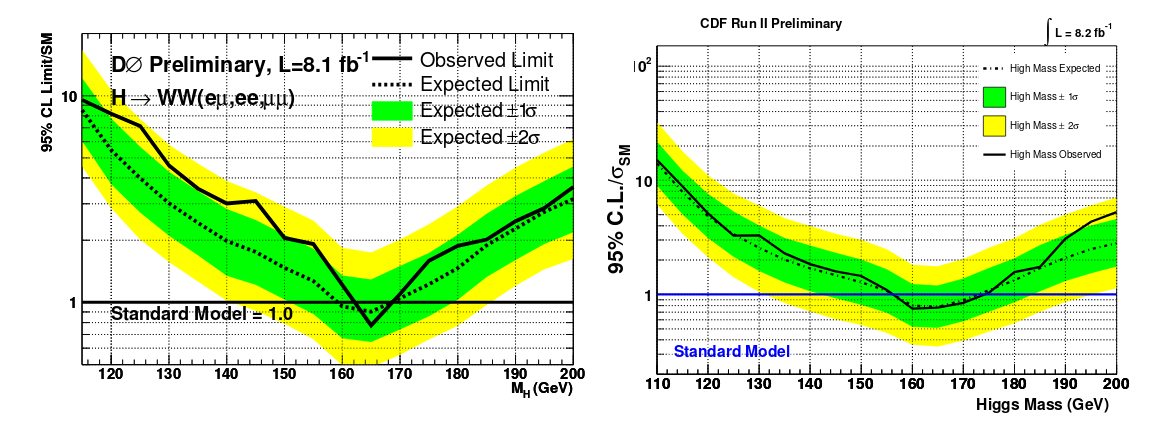
\includegraphics[scale= 0.33]{../Cap1/tevatron}
\caption{Combined limits using the di-lepton channels for D0 (left) and CDF (right).}
\label{tevatron}
\end{figure}

\paragraph{Searches at LHC} After the discovery of the Higgs boson at LHC, the two experiments, ATLAS and CMS, have been focused on high mass searches using the data collected at $\sqrt{s}=$7, 8 (Run-I) and 13 TeV (Run-II). A search for a heavy Higgs boson in the $H \to WW$ and $H \to ZZ$ decay channels has been performed by the
CMS experiment based on  proton-proton collision data samples corresponding to an integrated luminosity of up to 5.1 $fb^{-1}$ at $\sqrt{s}=7$ TeV and up to 19.7  $fb^{-1}$ at $\sqrt{s}=8$~\cite{Khachatryan:2015cwa}. This analysis is performed in a mass range 145 < $m_H$ < 1000 GeV and the heavy Higgs boson in the EW singlet extension of the SM. The peculiarity of this analysis is that the full Run-I statistics is considered and the mass range reach 1 TeV for the first time in CMS.
In the case of a high Higgs boson decaying into a pair of W bosons, the fully leptonic ($X \to WW \to 2\ell 2\nu$) and semileptonic ($X \to WW \to \ell \nu qq$) final
states are considered in this  analysis. For a high Higgs boson decaying into two Z bosons, final
states containing four charged leptons  ($X \to WW \to 2\ell 2\ell'$), two charged leptons and two quarks ($X \to ZZ \to \ell \nu qq$) and two charged leptons and two neutrinos ($X \to ZZ \to 2\ell 2\nu$) are considered. No significant excess over the expected
SM background has been observed and exclusion limits have been set. The combined results obtained for a heavy Higgs boson with SM-like couplings for all
the different contributing final states are displayed in Fig.~\ref{plots_combination_combinedSM_def}. On the left, the observed
95\% CL limit is shown for each final state. On the right, the expected and observed limits are
displayed for each of the individual channels as well as the combined result.
\begin{figure}
\centering
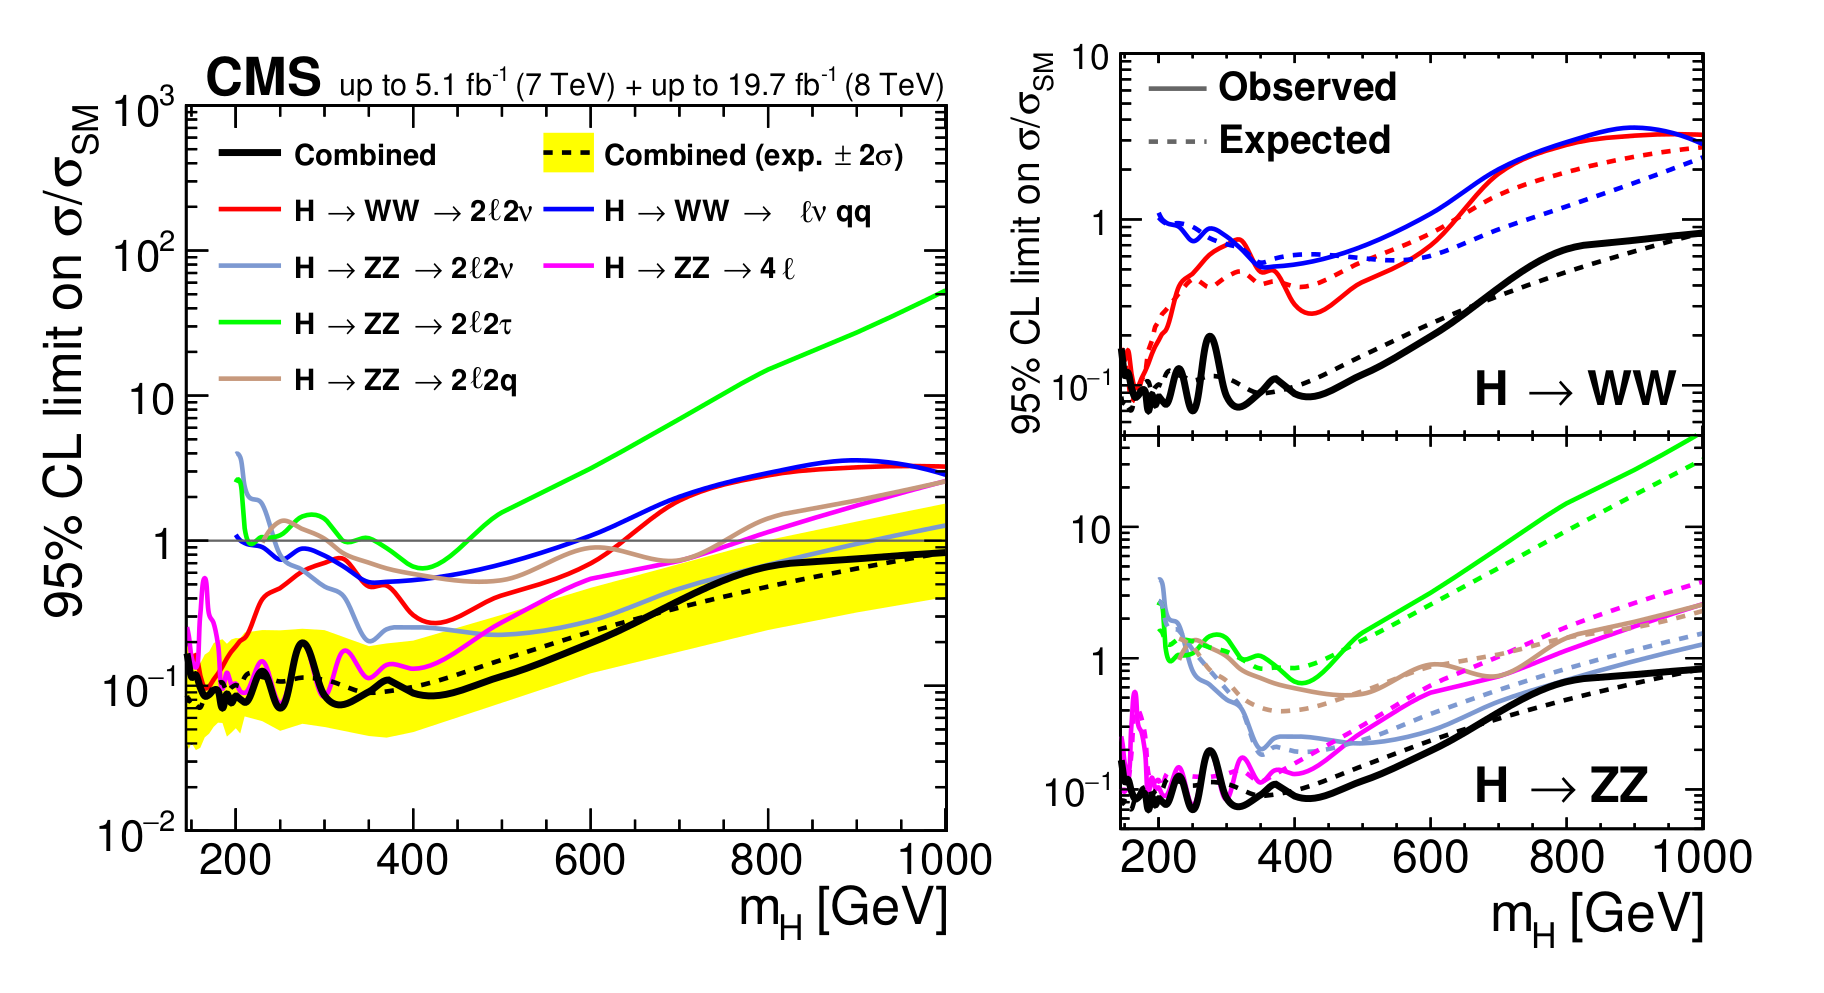
\includegraphics[scale= 0.9]{../Cap1/plots_combination_combinedSM_def}
\caption{Upper limits at the 95\% CL for each of the contributing final states and their combination. }
\label{plots_combination_combinedSM_def}
\end{figure}
Using the 13 TeV proton-proton collision data produced at the LHC in 2015, corresponding to an integrated luminosity
of 2.3 fb$^{-1}$, CMS has  performed the research of final state with different flavour leptons ($X \to WW \to 2\ell 2\nu$) in the range mass 200$< m_H< 1000$ GeV~\cite{CMS-PAS-HIG-16-023}. The search has been carried out in the 0-jets, 1-jet and VBF categories in order to increase the signal sensitivity to different production mechanisms and maximize the exclusion limits. The exclusion limits on the cross section times branching ratio to  WW $\to 2\ell 2\nu$ ave been reported and no significant excess with respect to the SM background expectation has been observed, Fig.~\ref{lim_2015}.
\begin{figure}
\centering
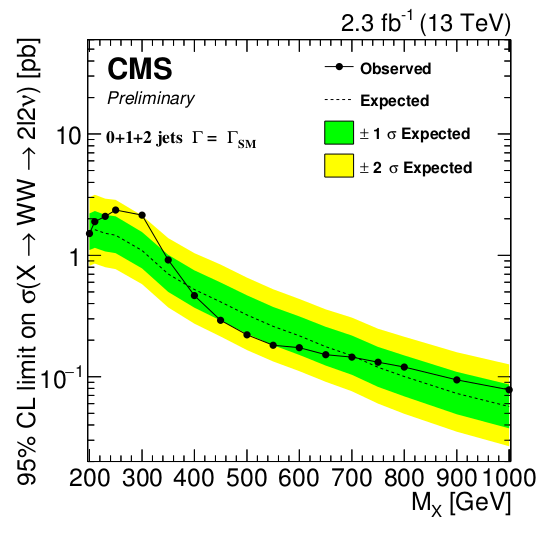
\includegraphics[scale= 0.4]{../Cap1/lim_2015}
\caption{Expected and observed exclusion limits at 95\% CL on the sum of ggH and VBF cross
sections times branching fraction for the combination of the three jet categories as a function
of the resonance mass. The black dotted line corresponds to the central value while the yellow
and green bands represent the $\pm 1\sigma$ and $\pm 2\sigma$  uncertainties respectively. }
\label{lim_2015}
\end{figure}
The ATLAS detector reported the results of a search for a heavy neutral scalar decaying to two W bosons using the datasets collected in 2015 and early
2016 at a centre-of-mass energy $\sqrt{s}=$13 TeV corresponding to an integrated luminosity of 13.2 fb$^{-1}$ in the mass range between
300 GeV and 3 TeV~\cite{ATLAS-CONF-2016-074}. In this analysis, categories with one- and at least two-jets
are optimised for a vector boson fusion-like signal and the remaining category is quasi-inclusive
for a gluon gluon fusion-like signal. The search sensitivity depends on the assumed Higgs boson width. Two different hypotheses are tested:
a narrow width approximation, where the width of the heavy Higgs boson is smaller than the
experimental resolution, and a large width assumption, where widths of 5\%, 10\%, and 15\% of
the heavy Higgs boson mass are considered.
Upper limits are set on the product of the production cross section and the $H \to WW$ branching ratio in two scenarios:
a high-mass Higgs boson with a narrow width, and one with intermediate widths (of 5, 10, 15\% of the
heavy Higgs boson mass), Fig.~\ref{ATLAS-CONF-2016-074_fig}. Values above 4.3 pb (1.4 pb) at $m_H=$300 GeV (400 GeV) and above 0.051 pb
(0.071 pb) at 3 TeV are excluded at 95\% CL by the gluon gluon fusion quasi-inclusive NWA (LWA 15\%) analysis. For
the VBF NWA case, the upper exclusion limit ranges between 1.1 pb at $m_H=$ 300 GeV to 0.03 pb at 3 TeV.

\begin{figure}
%\centering
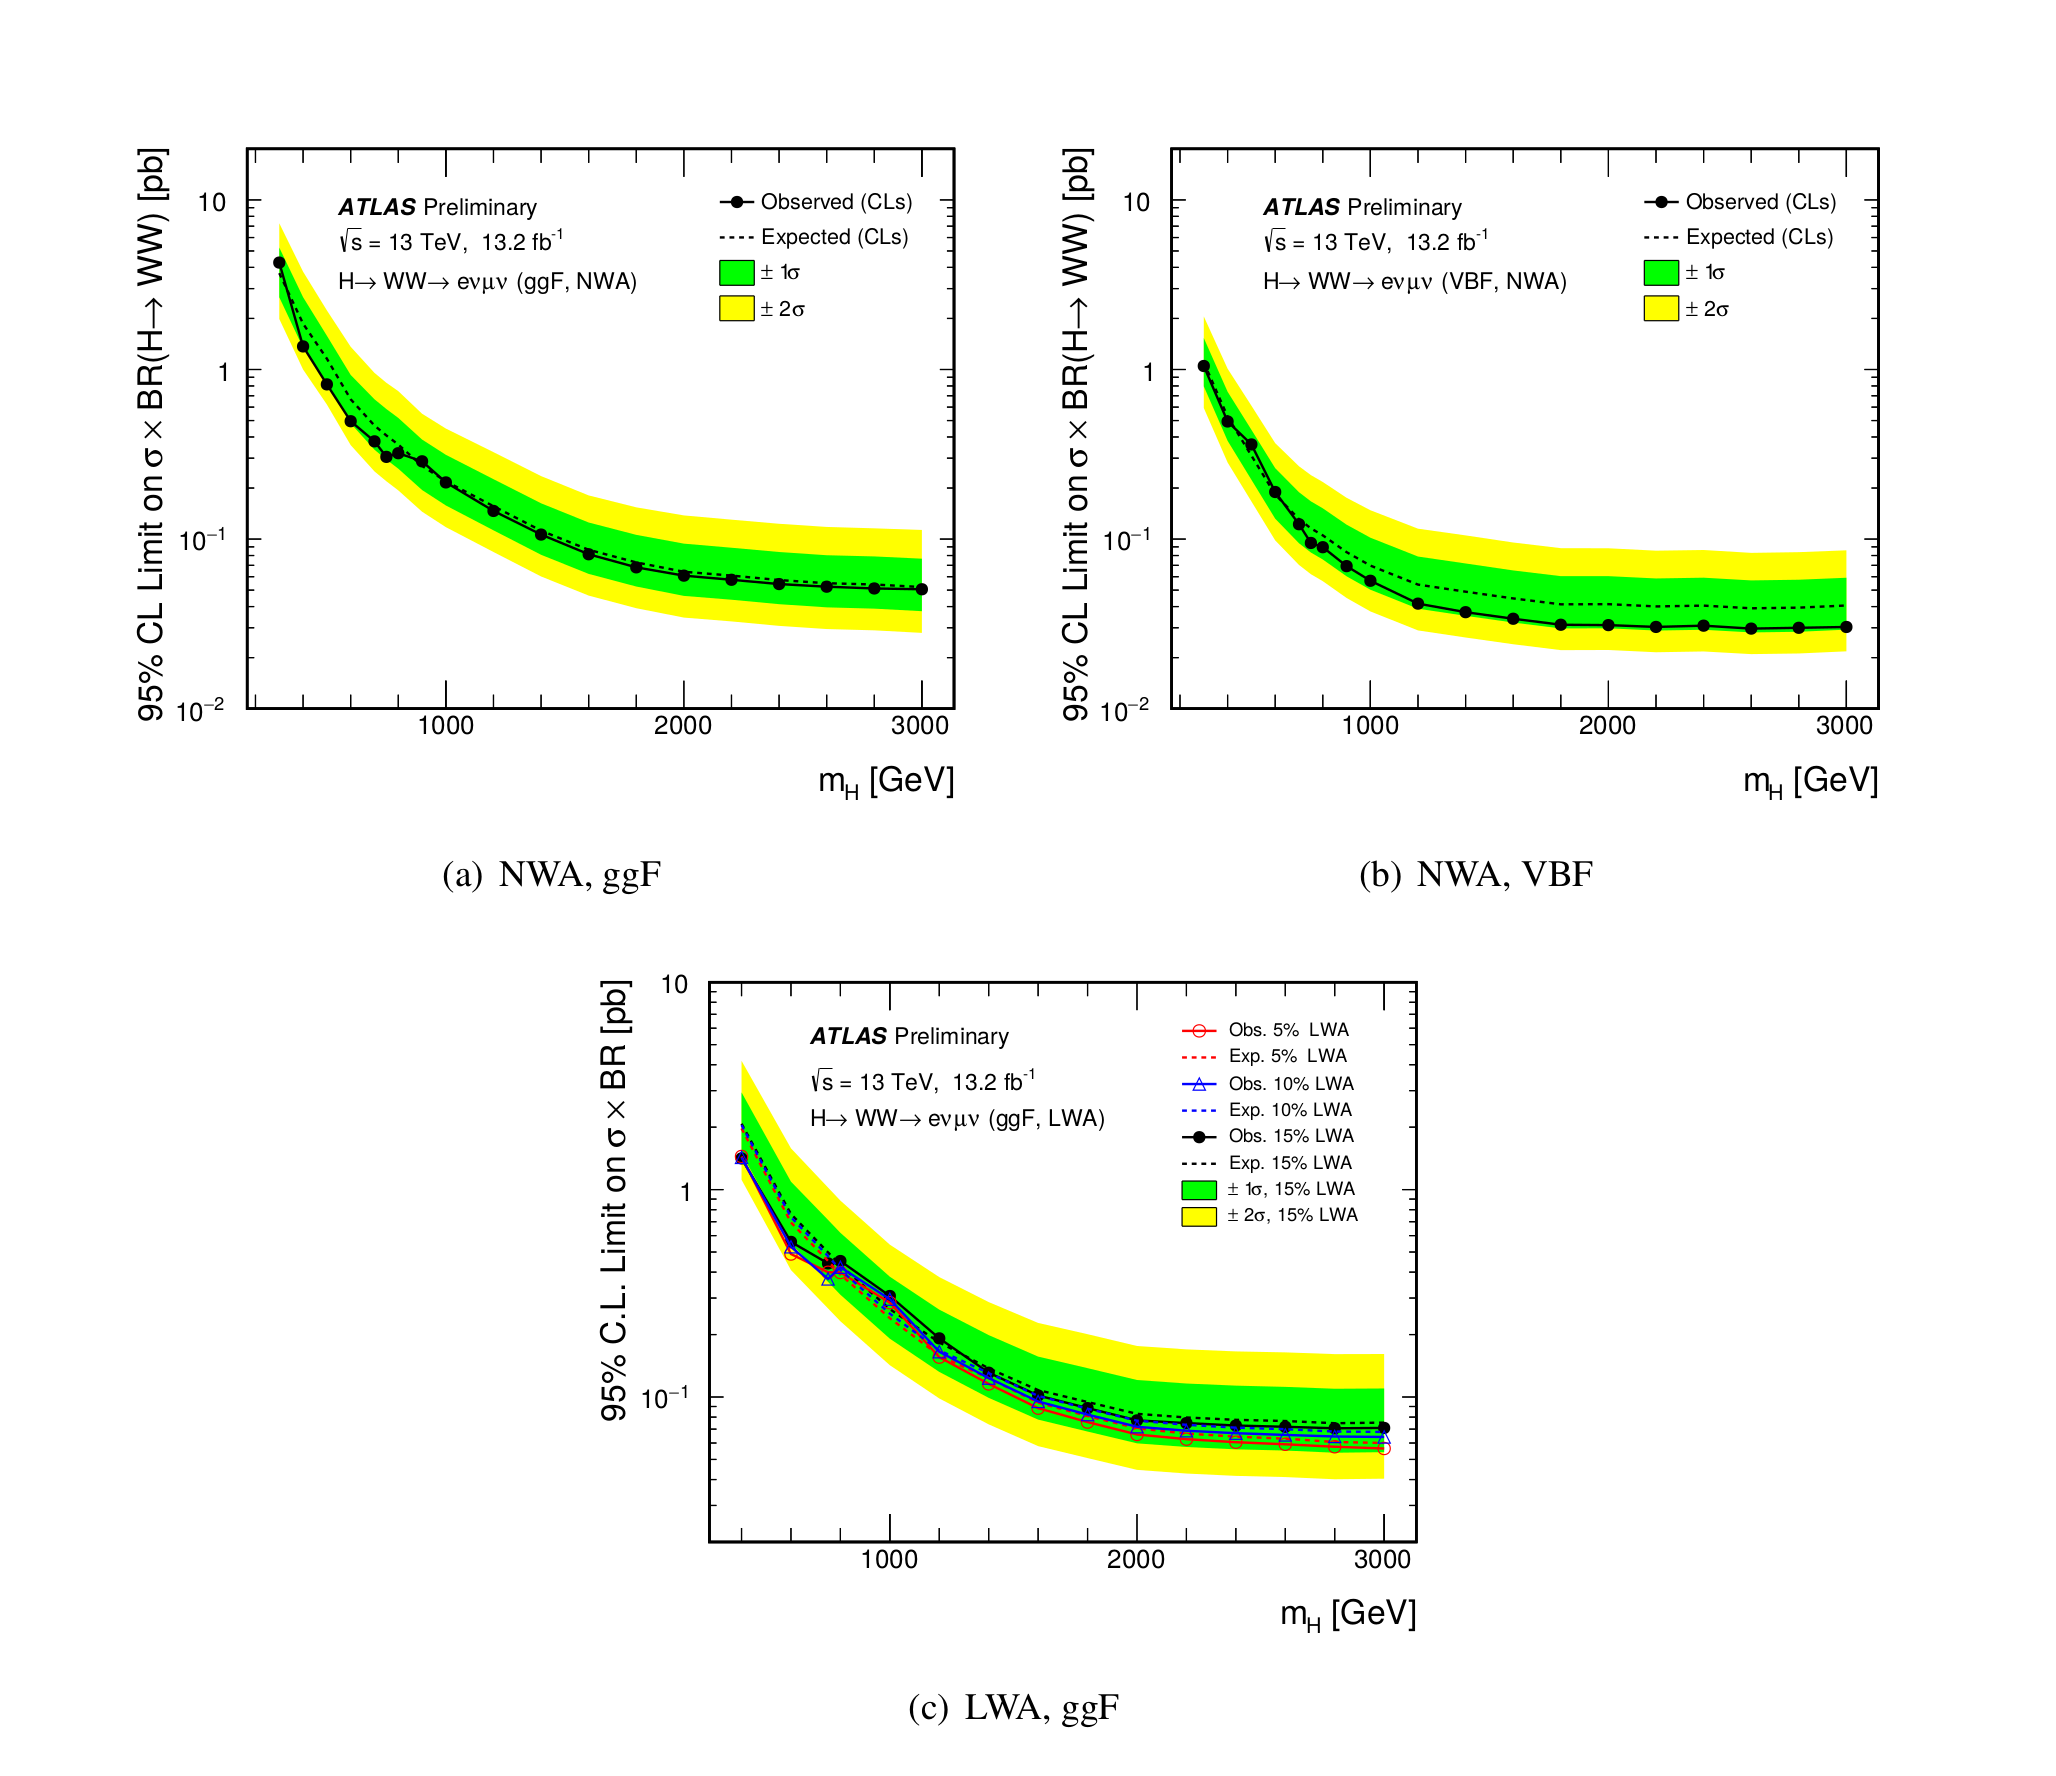
\includegraphics[scale= 0.9]{../Cap1/ATLAS-CONF-2016-074}
\caption{95\% CL upper limits on the Higgs production cross section times branching ratio in the analysis, for signals with narrow-width (gluon gluon fusion or VBF) in the top row and the 5\%, 10\% and 15\% width lineshapes (gluon gluon fussion only) in the bottom. The green and yellow bands show the  $\pm 1\sigma$ and  $\pm 2\sigma$ uncertainties on the expected limit. }
\label{ATLAS-CONF-2016-074_fig}
\end{figure}
